\subsection{Модификация закона Амдала (по проф. Бухановскому)}

В реальных вычислительных системах ОС тратит ресурсы на создание и удаление новых потоков. Время, затраченное на эти операции, не учитывается в законе Амдала. Параллельное ускорение $S(p)$ зависит от числа ядер и доли распараллеливаемых операций, но не зависит от числа последних. Выведем формулу, в которой число операций, для которых необходимо создать поток, будет учитываться.

Пусть $N$ -- число распараллеливаемых операций, $M$ -- число нераспараллеливаемых операций, $t_c$ -- время выполнения одной операции, $p$ -- число вычислителей (ядер), $T_i$ -- время выполнения программы при использовании $i$ параллельных потоков на $i$ вычислителях, $\alpha$ -- некий масштабирующий коэффициент, инкапсулирующий в себе время, требуемое на создание, удаление потока и прочие накладные операции. 
По формуле~\eqref{AmdalSFromP:equation}, $S(p) = {T_1} / {T_p}$.

Найдем сначала $T_1$. Так как это код выполняется линейно, то время, затраченное на его выполнение, будет равно числу операций, умноженному на время выполнения одной операции: $T_1 = t_c \cdot (N + M)$.

Время выполнения распараллельнной программы $T_p$ включает в себя время на создание потока: $t_c \cdot \alpha \cdot (p - 1) \cdot N$ (нужно создать $(p - 1)$ новых потоков, так как главный поток уже создан, и для каждого затратить какое-то время $\alpha$), время работы распараллеливаемоего кода на всех ядрах: $(t_c \cdot N) / {p}$ и время работы нераспараллеливаемого кода $t_c \cdot M$. Итого, разделив $T_1$ на $T_p$, получим формулу закона Амдала по проф. А.В. Бухановскому:

\begin{equation}
    \label{AmdalBuhunovsky:equation}
    S(p,N) = \frac{T_1}{T_p} = \frac{N + M}{\alpha \cdot (p - 1) \cdot N + \displaystyle\frac{N}{p} + M}.
\end{equation}

Из формулы~\eqref{AmdalBuhunovsky:equation} видно, что с ростом числа ядер после определенного предела $S(p,N)$  не будет расти как в законе Амдала, так как будет тратиться много времени на создание новых потоков. На рисунке~\ref{GraphAmdalBuhunovsky:image} наглядно видно, что $S(p,N)$ уменьшается при большом числе потоков и становится заметно меньше $S(p)$ по Амдалу даже при небольшом значении $\alpha$.

\begin{figure}[H]
    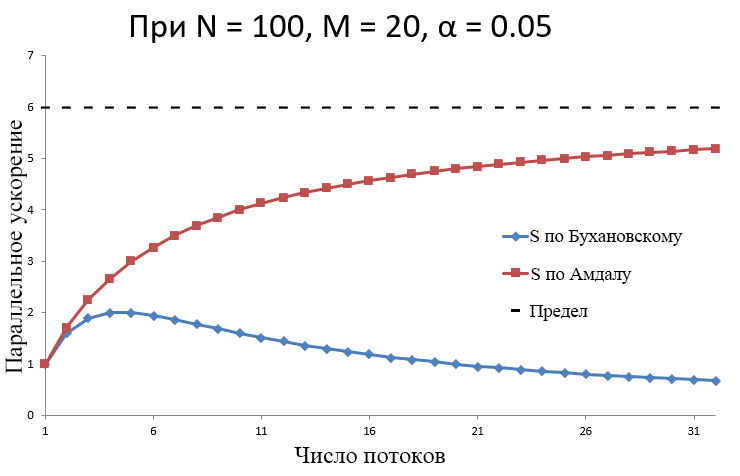
\includegraphics[width=\linewidth]{GraphAmdalBuhunovsky}
    \caption{График зависимости параллельного ускорения от числа потоков}
    \label{GraphAmdalBuhunovsky:image}
\end{figure}
